\chapter{Estudo de caso: A.M.I.G.O.S.}
\label{ap:estudo}

Nosso estudo de caso aplica-se sobre um ambiente digital de interação
desenvolvido para a gestão do conhecimento em rede social. Durante o estudo de
caso aplicamos a metodologia proposta no \chapref{ch:kddm} e seu passo a passo
será descrito nas seções \ref{ap:sec:dominio}, \ref{ap:sec:dados},
\ref{ap:sec:preparacao} e \ref{ap:sec:analise}. Nos resultados avaliaremos a
utilidade do método e das ferramentas desenvolvidas no processo.

\section{Entendendo o domínio}
\label{ap:sec:dominio}

Nosso objetivo neste processo de mineração é analisar uma ``fotografia'' do
ambiente digital do a.m.i.g.o.s. e extrair dela um grupo de atores-chaves;
aqueles que se destacam dos demais pelo seu posicionamento ou influência sobre a 
rede. Para darmos prosseguimento a análise, precisamos entender o ambiente e
decidir sobre a ferramenta de análsie que usaremos. Sobre o ambiente temos:

\begin{quote}{\citep{RicardoAraujoCosta2008}}
	Acrônimo de Ambiente Multimídia para Integração de Grupos e Organizações Sociais,
	o a.m.i.g.o.s tem por objetivo prover a infra-estrutura necessária para a criação
	de redes sociais virtuais para os mais diversos fins. Dentre estes, pode-se
	destacar o seu uso para estimular a criação e compartilhamento do conhecimento
	pelos seus diversos membros, podendo estes estarem relacionados a uma organização
	social. Nele é permitida a criação explícita das redes sociais através dos
	usuários e seus contatos. Cada contato é explicitamente adicionado por cada
	usuário, mesmo que dentro de uma mesma organização, e este relacionamento é
	navegável por qualquer outro membro da rede social. Nas próximas linhas são
	apresentadas as principais funcionalidades com suas características e possíveis
	usos.
	\begin{description}
	\item[Perfis] Cada usuário possui um perfil no a.m.i.g.o.s. Este perfil
	consiste de um conjunto de dados preenchidos na forma de cadastro, que definem
	algumas propriedades simples do usuário, como local de residência, idiomas que
	possui conhecimento, endereço de e-mail, identificadores de aplicações de
	mensagem instantânea (Windows Live Messenger, Skype, Google Talk, dentre
	outros), e uma descrição de suas áreas de interesse. Porém a parte mais
	relevante do perfil não é preenchida pelo usuário, e sim inferida pelo
	sistema. [\emph{Para cada usuário, um índice de atividade para a produção e
	consumo de conteúdos também é automaticamente calculado}]
	\item[Histórias] Histórias são destinadas ao registro, compilação e
	apresentação de conhecimentos emergentes entre os participantes da rede.
	Construído de forma gradual, através de contribuições espontâneas ou
	induzidas, qualquer usuário do sistema pode inserir no ambiente suas próprias
	histórias de sucesso ou dilemas, à medida que as considere relevantes para o
	objetivo da rede social. Adicionalmente as histórias podem estar associadas a
	uma ou mais comunidades, o que indica que, apesar do autor ser um usuário em
	específico, o conhecimento construído encontra-se de alguma forma relacionado
	a estas comunidades.

	Cada usuário do sistema poderá, adicionalmente, atuar como um revisor do
	conteúdo inserido por seus pares, avaliando qualitativamente as contribuições
	disponibilizadas neste ambiente. Esta avaliação pode ser realizada de uma das
	duas formas:
	\begin{itemize}
	  \item Adição de comentários que contribuam para a evolução da história,
	  criando-se assim uma história mais rica, com mais participantes e novos
	  conhecimentos. À medida que a história for acrescida de comentários, é criado
	  um diálogo associado ao conhecimento em construção;
	  \item Atribuição de uma nota, variando de uma (1) a cinco (5) estrelas, às
	  histórias que lê. Permitindo que este conhecimento, expresso através de
	  histórias, possa ser apresentado através de um ranking que indique as mais
	  relevantes para os membros daquela rede social.
	\end{itemize}
	\item[Relacionamentos] O a.m.i.g.o.s dá suporte a praticamente todos os
	mecanismos de relacionamentos existentes nas atuais redes sociais. Nele cada
	usuário pode adicionar a sua lista de contatos qualquer outro usuário também
	membro da rede social. Esta lista de contatos pode ser agrupada em grupos,
	facilitando a organização dos contatos pelo seu usuário.
	\item[Comunidades Virtuais] Comunidades podem ser vistas como agregações de
	pessoas com objetivos em comum. O a.m.i.g.o.s dá suporte à criação de
	manutenção de comunidades por parte de seus usuários, podendo estes convidarem
	membros de sua lista de contatos a participar das discussões ou atividades a
	serem realizadas no âmbito da comunidade.

	Cada comunidade possui uma série de mecanismos para a criação e
	compartilhamento do conhecimento. O principal mecanismo de criação e
	compartilhamento do conhecimento é o fórum de discussão, onde os membros da
	comunidade podem iniciar discussões sobre os mais diversos assuntos.

	Um segundo mecanismo de compartilhamento do conhecimento é a associação de
	histórias à comunidade. Esta associação pode ser realizada por qualquer membro
	da comunidade ao criar uma história no sistema. Caso deseje-se, é possível até
	mesmo que a história seja visível apenas pelos membros das comunidades
	relacionadas.
	\item[Recomendações] Como mecanismo de disseminação do conhecimento, o
	a.m.i.g.o.s possui suporte a recomendações. Estas recomendações são sempre
	direcionadas a usuários do sistema e podem ser referentes a histórias,
	comunidades, tópicos de um fórum ou outros usuários. Existem basicamente dois
	tipos de recomendação, uma feita manualmente por um usuário para seus
	contatos, e a outra realizada automaticamente pelo sistema para um usuário a
	partir da probabilidade do interesse deste no conteúdo recomendado.

	Para que a recomendação automática seja possível, o sistema vai montando o
	perfil do usuário à medida que este utiliza o sistema, baseado no que é lido ou
	escrito por ele. Para isto, o sistema faz uso do \emph{Vector Space Model}
	\citep{Barros2002}, varrendo o conteúdo textual disponível em cada elemento,
	calculando então o centróide do conteúdo e conseqüentemente o centróide do
	usuário, este composto pela soma vetorial do centróide de cada um dos seus
	conteúdos. Em seguida o sistema tenta identificar outros usuários ou conteúdos
	com centróides similares, recomendando-os ao usuário em questão sempre que
	esta similaridade for maior que um limiar configurado.
	\end{description}
\end{quote}

\begin{figure}[h!]
  \caption{\emph{Screenshot} da interface do A.M.I.G.O.S.}
  \centering
    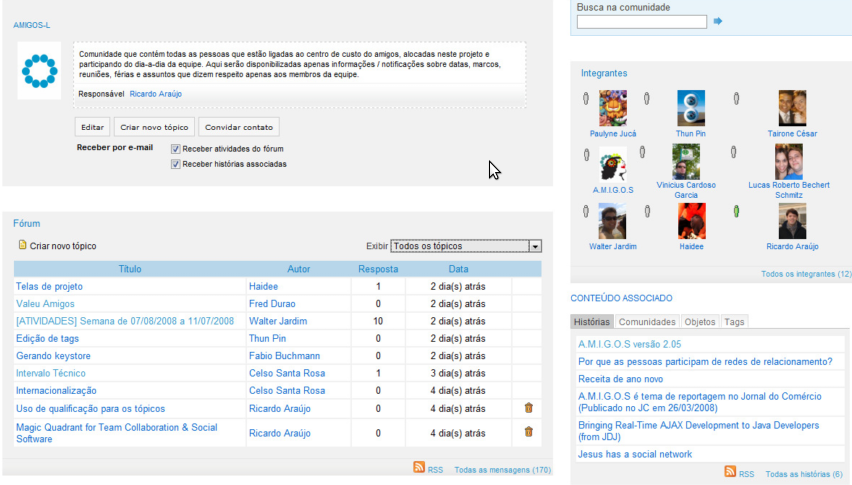
\includegraphics[width=0.7\textwidth]{imgs/screenshot-amigos.png}
    \label{ap:fig:screenshot}
\end{figure}

Considerando os critérios estabelecidos no \chapref{ch:dominio}, temos que a
representação da rede precisa ser não-binária e envolver a maior quantidade de
dimensões da força do laço possível; Por esta razão focaremos nas interações
textuais do a.m.i.g.o.s. usando o conceito de atenção apresentado na
\secref{sec:teoria_atencao}. Para a análise de influência, usaremos as métricas
de \emph{Flow betweenness} de \citeauthor{Freeman1991} e o poder de
\citeauthor{Bonacich1987}; as razões dessa escolha são a de que atendem aos
critérios de serem sensíveis tanto à estrutura macro da rede, quanto a
configuração local do nó, e também por simplicidade de implementação.

\section{Entendendo os Dados}
\label{ap:sec:dados}

Como para os fins desse estudo nos foi cedido o acesso a uma ``fotografia'' do
banco de dados do ambiente, então será uma análise intrínseca; não precisaremos
de \emph{crawlers}. Devido à complexidade de implementar algoritmos de análise de
sentimento, seguiremos uma abordagem ingênua e não consideraremos a intenção da
interação. Como se trata de interações em um contexto organizacional fechado, é
pouco provável que tenhamos disruptores e históricos longos de adversidade, de
forma que podemos considerar que muitas interações entre dois membros é uma bom
indicativo da positividade de suas intenções.

O poder da abordagem apresentada na \secref{sec:teoria_atencao} é a integração
de vários tipos de interação, conquanto sejam textuais. Então utilizaremos
quatro medianeiros textuais reconhecidos no ambiente e classificaremos de
acordo com a tipologia apresentada na \secref{sec:tipologia}:

\begin{description}
\item[Tópicos] são mensagens que \textbf{iniciam} discussões nos fóruns das
comunidades. A abrangência é individual desenvolvida, já que é direcionada aos
membros daquela comunidade apenas.
\item[Respostas] compõem o resto das mensagens nas discussões dos fóruns e
seguem naturalmente os tópicos e umas às outras. A abrangência também é
individual desenvolvida.
\item[Histórias] que são os textos de propósito geral que podem ser visualizados
por qualquer pessoa dentro do sistema, com algumas exceções. A abrangência,
nesse caso, pode ser individual desenvolvida quando relacionada a uma comunidade
apenas ou individual generalizada quando para todo o ambiente.
\item[Comentários] relativos às histórias publicadas. Cada história tem um
espaço público onde qualquer membro pode ler e publicar sua opinião, trata-se
portanto de uma interação de abrangência comum.
\end{description}

É importante denotar a abrangência de cada medianeiro pois que afeta diretamente
o cálculo da atenção reflexiva que cada autor tem com seus leitores. Usaremos o
coeficiente $\beta$ igual ao inverso multiplicativo da quantidade de membros da
abrangência, assim cada autor cede parcelas iguais a sua audiência por cada
interação. Para interações de abrangência generalizada para todo o ambiente, como
é o caso da grande maioria das histórias cadastradas, temos que $\beta=0$, por
tanto, o autor não cede atenção reflexiva para ninguém.

Como nossa anális é intrínseca, pela disposição da informação no banco de dados
podemos saber exatamente qual membro acessou e leu quais tópicos e histórias.
Por esta razão, definimos o coeficiente $\alpha$ da seguinte maneira: 0, caso
não tenha lido; $0.2$, caso tenha. Sendo assim, membros da abrangência que não
leram não cedem atenção ao autor, membros que leram cedem 20\% do total possível
e aqueles que leram e responderam ou comentaram cedem 100\% da atenção.

Fizemos $\gamma=^1/_2$ de forma que a atenção transitiva decai para a metade a
cada elo da \textit{thread}. Infelizmente, mesmo a análise sendo intrínseca, não
tivemos acesos a interações passivas do usuário como, por exemplo, o tempo que
ele passou em cada leitura ou logado no sistema. Dessa forma é complicado
estimar uma função de participação $E(.)$, porém nós podemos considerar o
próprio índice de atividade calculado pelo sistema como aproximação desse
parâmetro.

\section{Preparando os dados}
\label{ap:sec:preparacao}



\def \tick{
$[$\hspace{0.3cm}$]$
}

\def \twooption#1#2{
\tick #1.  \tick #2.
}

\def \threeoption#1#2#3{
\tick #1.\newline
\tick #2.\newline
\tick #3.
}

\def \fouroption#1#2#3#4{
\tick #1.\newline
\tick #2.\newline
\tick #3.\newline
\tick #4.
}

\def \fiveoption#1#2#3#4#5{
\tick #1.\newline
\tick #2.\newline
\tick #3.\newline
\tick #4.\newline
\tick #5.
}
\def \datefield{
%date fied used in time sheets
    /\hspace{0.4cm}/
}

\def \rcolor{
%table row color
    \rowcolor[gray]{0.9}
}

\def \hcolor{
    \rowcolor[gray]{0.7}
}

\section{Time sheet}
\label{ap:sec:time-sheet}

\begin{table*}[h]
  \centering
  \begin{tabular}{|c|c|c|c|c|p{5cm}|}
    \hline
    \hcolor ID & $Start~date$ & $Start~time$ & $End~date$ & $End~time$ & 
        $Is~it~a~duplicate?$\\
    \hline
       1 & \datefield  & : & \datefield & : & \twooption{Yes}{No} ID:\\
    \hline
       \rcolor 2 & \datefield  &  : & \datefield & : & \twooption{Yes}{No} ID:
       \\
    \hline
       3 & \datefield  &  : & \datefield & : & \twooption{Yes}{No} ID:\\
    \hline
       \rcolor 4 & \datefield  &  : & \datefield & : & \twooption{Yes}{No} ID:\\
    \hline
       5 & \datefield  &  : & \datefield & : & \twooption{Yes}{No} ID:\\
    \hline
       \rcolor 6 & \datefield  &  : & \datefield & : & \twooption{Yes}{No} ID:\\
    \hline
       7 & \datefield  &  : & \datefield & : & \twooption{Yes}{No} ID:\\
    \hline
       \rcolor 8 & \datefield  &  : & \datefield & : & \twooption{Yes}{No} ID:\\
    \hline
       9 & \datefield  &  : & \datefield & : & \twooption{Yes}{No} ID:\\
    \hline
       \rcolor 10 & \datefield  &  : & \datefield & : & \twooption{Yes}{No} ID:\\
    \hline
        \multicolumn{6}{|c|}{\ldots}\\
    \hline
       23 & \datefield  &  : & \datefield & : & \twooption{Yes}{No} ID:\\
    \hline
       \rcolor 24 & \datefield  &  : & \datefield & : & \twooption{Yes}{No} ID:\\
    \hline
       25 & \datefield  &  : & \datefield & : & \twooption{Yes}{No} ID:\\
    \hline
       \rcolor 26 & \datefield  &  : & \datefield & : & \twooption{Yes}{No} ID:\\
    \hline
       27 & \datefield  &  : & \datefield & : & \twooption{Yes}{No} ID:\\
    \hline
       \rcolor 28 & \datefield  &  : & \datefield & : & \twooption{Yes}{No} ID:\\
    \hline
       29 & \datefield  &  : & \datefield & : & \twooption{Yes}{No} ID:\\
    \hline
       \rcolor 30 & \datefield  &  : & \datefield & : & \twooption{Yes}{No} ID:\\
    \hline
       31 & \datefield  &  : & \datefield & : & \twooption{Yes}{No} ID:\\
    \hline
       \rcolor 32 & \datefield  &  : & \datefield & : & \twooption{Yes}{No} ID:\\
    \hline
  \end{tabular}
\caption{Time sheet used in the study.
%The subjects use this time
%sheet to note the start and end timestamps of a bug-report analysis, and mark
%if has been found a duplicate for the bug-report under analysis.
}
\end{table*}

\newpage
\section{Questionnaire for Subjects Profile}
\label{ap:sec:profile}

\begin{table}[h]
\centering
\resizebox{15cm}{!}{
\begin{tabular}{|p{\columnwidth}|}
    \hline
    \hcolor \textbf{\textsf{Questionnaire for Subjects Profile}}\\
    \hline
	    \textbf{How many years since graduation?}\\\\
	    \tick years.\\\\
    \hline
        \textbf{How many projects do you have participated according to the
        following categories?}\\ \\
        \tick Low complexity.\\
        \tick Medium complexity.\\
        \tick High complexity.\\\\
    \hline
        \textbf{What were the roles that you played in the projects cited before
        (developer, configuration manager, tester\ldots)?}
        \\
        \\
    \hline
        \textbf{How do you define your experience with bug-trackers?}\\\\
        \tick I never used them before.\\
        \tick I used them in every project i participated.\\
        I used them in \tick projects.\\\\
    \hline
        \textbf{Do you have used any of the following bug-trackers?}\\\\
        \tick Bugzilla. In: \tick industry  \tick academia\\
        \tick Trac. In: \tick industry  \tick academia\\
        \tick Mantis. In: \tick industry  \tick academia\\
        \tick Jyra. In: \tick industry  \tick academia\\
        \tick BSD Bug-tracker. In: \tick industry  \tick academia\\
        \tick Other: \\\\
    \hline
        \textbf{Have you performed any analysis of Firefox bug-reports before?}
        \\\\\twooption{Yes}{No}\\\\
    \hline
\end{tabular}
}
\caption{Questionnaire for bug-report submitters.}
\end{table}

\newpage
\section{Form for Qualitative Analysis}
\label{ap:sec:feedback}

\begin{table}[h]
\centering
\resizebox{14cm}{!}{
\begin{tabular}{|p{\columnwidth}|}
    \hline
    \hcolor \textbf{\textsf{Questionnaire for Qualitative Analysis}}\\
    \hline
        \textbf{Did you use any of the search filters provided by BAST?}
        \\
        \twooption{Yes}{No}
        \\
    \hline
        \textbf{Is there any search filter you think it must be present in BAST?}
        \\
        \twooption{Yes}{No}
        Cite them:
        \\
    \hline
        \textbf{Did you have any problem with the search filters usage?}
        \\
        \twooption{Yes}{No}
        Cite them:
        \\
    \hline
        \textbf{Did you use the ordering features of BAST?}
        \\
        \twooption{Yes}{No}
        \\
    \hline
        \textbf{Did you have any problem with ordering features?}
        \\
        \twooption{Yes}{No}
        Cite them:
        \\
    \hline
        \textbf{Do you think there is any other important information that
        must be present in the list of search results?}
        \\
        \twooption{Yes}{No}
        Cite them:
        \\
    \hline
        \textbf{Did you have any problem to visualize the details from some
        bug-report?} \\
        \twooption{Yes}{No}
        Cite them:
        \\
    \hline
        \textbf{Do you believe the way bug-reports details are presented was
        helpful to perform the analysis?}
        \\
        \twooption{Yes}{No}
        \\
    \hline 
        \textbf{Was the recommendation of related bug-reports, presented  in
        the bug-report details, useful for the analysis?}
        \\
        \twooption{Yes}{No}
        \\
    \hline
        \textbf{Is there any other information concerning bug-reports details
        you believe it should be present or emphasized?}
        \\
        \twooption{Yes}{No}
        Cite them:
        \\\\
    \hline
        \textbf{Did you use the help provided by BAST?}
        \\
        \twooption{Yes}{No}
        \\
    \hline
        \textbf{Did you found any other problem/enhacement/defect that was not
        mentioned before? Cite them.}
        \\
        \\
        \\
    \hline
        \textbf{Please, write down any suggestion you think might would be useful.}
        \\
        \\
        \\
    \hline
\end{tabular}
}
\caption{Questionnaire for qualitative analysis.}
\end{table}